%!TEX root = ../template.tex
%%%%%%%%%%%%%%%%%%%%%%%%%%%%%%%%%%%%%%%%%%%%%%%%%%%%%%%%%%%%%%%%%%%%
%% chapter2.tex
%% NOVA thesis document file
%%
%% Chapter with the template manual
%%%%%%%%%%%%%%%%%%%%%%%%%%%%%%%%%%%%%%%%%%%%%%%%%%%%%%%%%%%%%%%%%%%%
\chapter{Related Work}
\label{cha:related_work}

% ================
% = Introduction =
% ================
We’re currently in a period where we start to depend more and more on allowing remote services to access our data and execute our applications. Cloud computing systems require users to trust them with their data. Therefore these systems need a way to assure data privacy
and security, thus gaining users trust.

In this chapter we address existing solutions that are able to protect applications from the \gls{os} or hypervisor, regardless the machine where they're running on, thus increasing the level of trust an user can deposit in an execution of an application.

These existing solutions are organized in different sections in the following way: 
Section 2.1 covers protection against untrusted \gls{os}es; 
Section 2.2 covers \gls{tee}s and hardware-enabled approaches;
In Section 2.3 we cover, in more detail, hardware-enabled \gls{tee} solutions used today.
Section 2.4 covers shielded applications and frameworks compatible with Intel-\gls{sgx}, which is the \gls{tee} technology we choose for our approach.
Finally, in Section 2.4 we make a critical analysis on the topics previously discussed, while covering their main advantages and disadvantages.





\section{Protection in untrusted OSes}

A lot of applications these days depend on sensitive data to operate. Therefore protecting this data must be taken into account while designing the application. 
One of the things we have to think about is the size of the TCB, and how to reduce it as much as possible without losing the operability of the system. 
Typically, the host OS is considered safe and trustworthy, although that is not always the case. A compromised OS can give complete access to sensitive data, if not isolated from the application. That’s why this is a major security problem and must be tackled in today’s systems.

Approaches like Virtual Ghost \cite{virtGhostPaper}, Flicker \cite{flickerPaper}, MUSHI \cite{mushiPaper}, SeCage \cite{SeCagePaper}, InkTag \cite{inkTagPaper}, Sego \cite{segoPaper}, grant security by isolating the sensitive data from the untrusted \gls{os} either by monitoring the application while it runs, or by enforcing memory isolation by using virtualization.


-------------------------- TO DO -----------------------------

			drawback of those approaches (inktag, virtghost...)
			and why aren't enough
			
-------------------------- END OF TO DO -----------------------------



\section{Hardware-Enabled TEE - Trusted Execution Environments}

A \gls{tee} is an abstraction provided by both software and hardware that guarantees isolated execution of specific programs in a machine, including the host \gls{os}, hypervisor or even system administrators, preventing them from leveraging their priviledges. A \gls{tee} also provides integrity of applications running inside it, along with confidentiality of their assets.

The first attempts to implement a \gls{tee} on a cloud system consisted of combining a hypervisor with isolation properties and a \gls{tpm}. 

A \gls{tpm} \cite{tpmPaper} consists of a hardware chip, called microcontroller, that aims to create a trustable platform, through encryption and authenticated boot, and make sure it remains trustworthy, through remote attestation. 
It provides cryptographic functions that can't be modified, and a private key (Endorsment Key) that is unique to every \gls{tpm} made, working as an identifier for each \gls{tpm}.

However, \gls{tpm}s have several problems when applied to the cloud due to being designed with the intention to offer security to a single machine. Thus, a distributed environment would not be the best kind of environment for a \gls{tpm} to work on.

With that in mind, new hardware-enabled solutions were developed to be more flexible and cloud friendly than the \gls{tpm}. Technologies like ARM TrustZone, Intel SGX, AMD-SEV, and others, will be approached in the following section.

-------------------------- TO DO -----------------------------

 			should we talk about HSM ?????

-------------------------- END OF TO DO -----------------------------

\section{Hardware-Enabled TEE Solutions}


The idea of using hardware to provide trusted execution environments started appearing as a way to deal with piracy, with examples like TCPA \cite{tcpaPaper} and Microsoft's Palladium being the most known ones. By making use of hardware, it was possible to encrypt data (DVD's, for example) that could only be decrypted by a specific hardware, making it impossible to copy. 

Although this approaches were effective back in the day, both of them place their trust in the hardware, not trusting the \gls{os} entirely. 
Thus, since any application does not trust the \gls{os}, it does not trust the application to properly use its resources either. Therefore, some of the protection aspects of the \gls{os} must be moved into the hardware, as well as changing the interface between the \gls{os} and the application so it supports the hardware security features.

XOM \cite{xomPaper}, described in the next subsection, was developed as a way to deal with these changes that were required to use this idea of trusted computing in a better way.


\subsection{XOM}




-------------------------- TO DO -----------------------------



XOM | a processor architecture that provides
copy protection and tamper-resistance functions. In XOM,
only the processor is trusted; main memory and the operat-
ing system are not trusted. 

Our operating system (XOMOS) manages hardware
resources for applications that don't trust it. This requires a
division of responsibilities between the operating system and
hardware that is unlike previous systems.

There are several good reasons for creating tamper-res-
istant software including enabling
mobile code to run on untrusted platforms without the risk
of tampering or intellectual property theft, and enabling the
deployment of trusted clients in distributed services such as
banking transactions, on-line gaming, electronic voting, and
digital content distribution.

Tamper-resistance can be enforced using software or hardware techniques

Trusting the hardware rather than the software has in-
teresting implications for operating systems design. Since
sharing hardware resources among multiple users is a di-
cult task, often requiring complex policy decisions, it is most
naturally done in software by an operating system.

This paper explores the design of an operating system that
runs on hardware that supports tamper-resistant software.

Our operating system is intended to work with an existing
processor architecture called XOM, which stands for eXe-
cute Only Memory [17]. In the XOM processor architec-
ture, programs do not trust the operating system or external
memory, but instead, trust the processor hardware to pro-
tect their code and data.

XOM can protect against a sophisticated attacker who may have physical access to the hardware

The XOM attack model also assumes that main memory may be compromised by an adversary. The XOM processor
not only encrypts values in memory, but also stores hashes of
those values in memory as well.
It will only accept encrypted values
from memory if accompanied byavalid hash.

Currently, there exist various initiatives that place the
trust in modern computing systems in an hardware component rather in the OS
In these systems,
the applications don't trust the operating system to protect
their data, but the operating system also does not trust the
application to properly use its resources.
As a result the interface between the operating system and applications must change to support the hardware security features, and some of the protection aspects of the operating system must
be moved into the hardware.
This paper studied how these
changes can be implemented and what the impact of those
changes on the performance of the system is.
 
-------------------------- END OF TO DO -----------------------------

\subsection{ARM TrustZone}
\label{ssec:armtz}

ARM Trust Zone \cite{armTZPaper} are hardware security extentions offered by ARM application processors with the same finality as Intel \gls{sgx}, create isolated environments where software can execute in a secured and trustable way. 

To accomplish this, ARM processors implement two virtual processors backed by hardware access control, where the software stack can switch between two states called secure world (SW) and normal world (NW). 
The first one has higher priviledges than the second one, therefore it can access NWs copies of registers, but not the other way around. SW is also responsible of protecting running processes in the \gls{cpu}, while providing secured access to peripherals. 
Each world acts like a runtime environment and has it's own set of resources. This resources can be partioned between the two worlds or just assigned to one of them, depending on the ARM chip specs.

For the context switch between worlds, ARM processors implement a secured mode called Secure Monitor, where there's a special register responsable of determine if the processor runs code in SW or NW. 

Most ARM processors also offer memory curtaining. This consists on the Secure Monitor allocating physical addresses of memory specifically to the SW, making this region of memory unaccessible to the rest of the system.

By default, the system boots always in SW so it can provision the runtime environment before any untrusted code start to run. It eventually transitions to NW where untrusted code can start to be executed. 

\subsection{AMD-SEV}
\label{ssec:amdsev}
AMD Secure Encrypted Virtualization (SEV) is the AMD approach to provide a \gls{tee}, integrated with virtualization. It's a technology focused primarily on cloud computing environments, specifically in public \gls{iaas}, as its main goal is to reduce trust from higher priviledged parties (\gls{vmm}s or \gls{os}), so that they can not influence the execution on the other "smaller" parties (\gls{vm}s). 

To achieve this, AMD grants encryption of memory through a technology called Secure Memory Encryption (SEM), or through TransparentSEM (TSEM) if the system runs a legacy OS or hypervisor with no need for any software modifications.
After the data is encrypted, SEV integrates it with AMD virtualization architecture to support encrypted \gls{vm}s. By doing this, every \gls{vm} is now protected from his own hypervisor (\gls{vmm}), unabling its access to the decrypted data. Although uncapable of accessing the \gls{vm}, the \gls{vmm} is still responsible of controlling each \gls{vm}'s resources. \cite{amdPaper}

Thus, AMD provides confidentiality of data by removing trust from the \gls{vmm}, and creates an isolated environment for the \gls{vm} to run, where only the \gls{vm} and the processor can be trusted. However it does not provide integrity of data, allowing replaying attacks to take place, and has a considerably large \gls{tcb}, since the \gls{os} of each \gls{vm} is trusted. \cite{amdSEVPaper}

\subsection{Sanctum}
\label{ssec:sanctum}
Just like \gls{sgx}, the main objective of Sanctum is to offer strong isolation of software modules, altough following a different approach focused in avoiding unnecessary complexity, thus granting a simple security analysis.
To make this possible, Sanctum \cite{sanctumPaper}, which tipically runs in a RISC-V processor, combines minimal and minimally invasive hardware modifications with a trusted software security monitor that is receptive to analysis and does not perform cryptographic operations using keys. 

This minimality idea consists on reusing and slightly modifying existing well-understood mechanisms, while not modifiying \gls{cpu} building blocks, only adding hardware to the interfaces between blocks, causing Sanctum to be adaptable to other processors in addition to RISC-V. 

Sanctum is a pratical approach that shows that a strong software isolation is achievable with a small set of minimally invasive hardware changes, causing reasonably low overhead. 
This approach provides strong security guarantees dealing with side-channel attacks, such as cache timing and passive address translation attacks.

\subsection{Intel-SGX}
\label{ssec:intelsgx}
Intel Software Security Guard Extensions (SGX) are a set of instructions built in Intel \gls{cpu}s, that allow programmers to create \gls{tee}s, called enclaves. Enclaves are isolation containers that create an isolated environment where sensitive code can be stored and executed inside, ensuring integrity and confidentiality to it. By doing so, it reduces the \gls{tcb} in a way that most of the system software, apart from the enclaves and the \gls{cpu}, is considered not trusted.

Enclaves are mapped into private regions of memory, where only the \gls{cpu} has access to, reducing the \gls{tcb} to only the enclave and the \gls{cpu} itself. Due to this restrictions, not even the most common system libraries can be accessed inside the enclave, since the \gls{os} is not considered trusted. 

A system that encorporates \gls{sgx} under it's architecture is divided in two: a trusted component being the enclave, and an untrusted component being the rest of the system. The untrusted one requests the launch of the enclave, where the \gls{cpu} then manages to allocate the enclave in a private region of memory, made available only to that particular enclave. This portion of memory is kept encrypted in volatile memory, being only decrypted by the \gls{cpu} if the responsible enclave requests it \cite{guiBorgesThesis}.

Altough isolation is the main objective of \gls{sgx}, it still allows a way for both  untrusted and trusted parties to communicate. This is made possible by the functions ECALL and OCALL. ECALLs are used for an untrusted component to call for trusted code in a secured way - the enclave copies the pointers to that specific code into a buffer, which is then made visible for the untrusted component, ensuring that the untrusted party can't know the real memory address inside the enclave. To communicate the other way arround the enclave calls for an OCALL, where the enclave is temporarily exited, executing then the unstrusted function needed. After that, the enclave is re-entered. OCALLS are mainly used by the enclave to access the network or to deal with I/O disk access.

\section{SGX-Enabled Frameworks and Shielded Applications}
\subsection{Shielded protected applications in untrusted Clouds}

-------------------------- TO DO -----------------------------



-------------------------- END OF TO DO -----------------------------

\subsection{SCONE}

-------------------------- TO DO -----------------------------



-------------------------- END OF TO DO -----------------------------

\subsection{Haven}

-------------------------- TO DO -----------------------------



-------------------------- END OF TO DO -----------------------------

\subsection{OpenSGX}

-------------------------- TO DO -----------------------------



-------------------------- END OF TO DO -----------------------------

\subsection{Panoply}

-------------------------- TO DO -----------------------------



-------------------------- END OF TO DO -----------------------------

\subsection{VC3}
\label{ssec:vc3_mapreduce}

Verifiable Confidential Cloud Computing (VC3) \cite{vc3Paper} is a framework that achieves confidentiality and integrity of data, as well as verifiability of execution of code with good performance through MapReduce \cite{mapReduce} techniques. It uses Intel SGX processors as a building block and runs on unmodified Hadoop \cite{hadoop}.
In VC3 users implement MapReduce jobs, compile and encrypt them, thus obtaining a private enclave code E-. They then join it with a small portion of public code E+, that implements the protocols for key exchange and job execution.
Users then upload the resulting binary code to the cloud, where enclaves containing both E- and E+ are initialized by an untrusted framework F. 

\begin{figure}[htbp]
	\centering
	{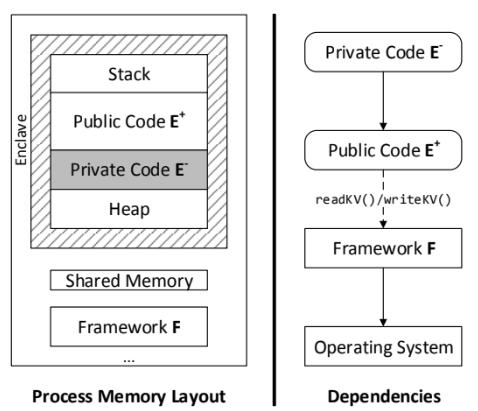
\includegraphics[width=0.6\linewidth]{vc3_design}}%
	\caption{VC3 memory design model on the left, component dependencies on the right}
\end{figure}

A MapReduce begins with a key exchange between the user and the E+ code running in the enclave. After this, E+ can proceed to decrypt E- and process the encrypted data. VC3 isolates this processing from the OS by keeping an interface between the E+ layer and the outside of the enclave. This interface consists of basically two functions: readKV() and writeKV(), for reading a key-value pair on Hadoop or write it, respectively. Also, the data inside of the enclave is passed to the outside, more specifically from E+ to the untrusted F, by using a virtual address space shared by both.
With VC3, both E- and the user data are always encrypted while in the cloud, except when processed by the trusted processor, while allowing Hadoop to manage the execution of VC3 jobs. Map and reduce nodes are seen as regular worker node to Hadoop, therefore Hadoop can provide its normal scheduling and fault-tolerance mechanisms, as well as load balancing. VC3 accomplishes this keeping Hadoop, the OS and the hypervisor out of the TCB.

\subsection{Protected Zookeeper}
\label{ssec:protected_zookeeper}

ZooKeeper \cite{zookeeper} is a replicated synchronization service for distributed systems with eventual consistency. However, ZooKeeper does not guarantee privacy of data stored inside of it by default.

Protected ZooKeeper \cite{protectedZooKeeper} is an approach that eliminates this privacy concerns, by placing an aditional layer between the client and the ZooKeeper, refered as ZooKeeper Privacy Proxy (ZPP). ZPP is a layer responsible for the encryption of all sensitive information, during a communication between a client and the ZooKeeper. 
Clients communicate with the proxy via a SSL connection, where the packets are encrypted by an individual session key. Here, ZPP acts like a normal ZooKeeper replica to the client. 
After receiving the packets from the client, ZPP extracts the sensitive data, encrypts it with a mechanism that allows the data to be decrypted by the proxy later on, and forwards the encrypted packet to a ZooKeeper replica where it can be stored with integrity ensured.

ZPP runs inside a TEE, located in the cloud, allowing it to store encryption keys and process plaintext data safely. As a result, even if the attacker is the cloud provider itself, the integrity of the data will still be granted since the attacker won't be able to access or alter anything running inside the TEE.

ZPP also retains all original ZooKeeper functionality, and does not affect ZooKeeper's internal behaviour. Therefore adapting existing ZooKeeper applications to this concept of ZPP it's easily done.

This approach allows applications in the cloud to use ZooKeeper without privacy concerns at the cost of a small decrease of throughput.
\subsection{Ryoan}
\label{ssec:ryoan_sandboxing}

Ryoan \cite{ryoanPaper} consists on a distributed sandbox that allows users to protect the execution of their data. This is achieved with the help of Intel SGX \cite{intelSGX} \cite{sgxPaper} enclaves, creating sandbox instances that protect data from untrusted software while also preventing leaks of data, which is a weakness of enclaves caused by side channel attacks.
Ryoan does not include any priviledged software (e.g. OS and hypervisor) in it's TCB, while trusting only the hardware (SGX enclave) to assure secrecy and integrity of the data.

It's main goal is to prevent leakage of secret data. This is done by preventing modules from sending sensitive data over their communications if outside the system boundaries, as well as eliminating stores to unprotected memory and system calls, made possible by the use of a trusted sandbox Native Client (NaCl). 

\begin{figure}[htbp]
	\centering
	{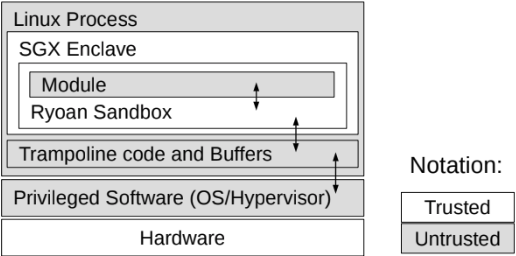
\includegraphics[width=0.6\linewidth]{ryoan_design}}%
	\caption{Instance of Ryoan running on a single machine}
\end{figure}

Ryoan's approach consists on confining the untrusted application in a NaCl, responsable of controlling system calls, I/O channels and data sizes. This NaCl sandbox is implemented inside the enclave, and can communicate with other instances of the NaCl, forming a distributed sandbox between users and different service providers. Inside the sandbox, the untrusted application can execute safely on secret data. The NaCl sandbox uses a load time code to ensure that the module can not do anything it shouldn't, thus violating the sandbox. To handle faults, exceptions or errors inside the NaCl sandbox, Ryoan uses an unprotected trampoline code, that can enter the enclave and read the information about the fault so it can handle it.
\subsection{Opaque}
\label{ssec:opaque}

Opaque \cite{opaquePaper} is a distributed data analytics platform that guarantee encryption, secure computation and integrity to a wide range of queries. Therefore, instead of being implemented in the application layer or the execution layer as this kind of security approaches usually are, Opaque is implemented in the query optimization layer. 

It is implemented with minimal modifications on Spark SQL, and uses Intel SGX technology as a way to grant confidentiality and integrity of the data. 
However, the use of enclaves can still be threatened by access pattern leakage that can occur at memory-level, when a malicious OS infers information about encrypted data just by monitoring memory page accesses, and at network-level, when network traffic reveals information about encrypted data.

Opaque hides access patterns in the system by using distributed oblivious relational operators and optimizes these by implementing new query planning techniques. It can be executed in three modes

\begin{itemize}
	\item encryption mode: provides data encryption and authentication, while granting correct execution.
	\item oblivious mode: provides oblivious execution, protecting against access pattern leakage.
	\item oblivious pad mode: extends the oblivious mode by adding prevention of size leakage.
\end{itemize}

Opaque is an approach that is able to grant oblivious execution 3 times faster than other specialized oblivious protocols.

\subsection{Graphene-SGX}
\label{ssec:grapheneSGX}

The usage of Intel SGX, and similar technologies, have proven to add a great sense of privacy to the storage and execution of data in applications. However this tecnologies impose restrictions (e.g., disallowing system calls inside the enclave) that require the applications to be changed so they can benefit from this extra layer of security. 

Graphene-SGX \cite{graphenePaper} came to help circunvent those restrictions, while still assure security to the data. It is a library OS that aims to reproduce system calls, respecting security concerns, so that unmodified applications can use them to keep executing normally without interacting directly with the OS or hypervisor. 

By using a library OS, the system is expected to lose performance and, since a new layer of software was added, to increase the size of the TCB. 
Although these assumptions are true, they are quite often exagerated. Graphene-SGX's performance goes from matching a Linux process to less than 2x in most executions of single-processes.
Graphene-SGX has also shown some great results comparing it to other similar approaches that use shim layers, such as SCONE \cite{sconePaper} and Panoply \cite{panoplyPaper}, where it shows to be performancewise similar to SCONE and faster 5-10 percent than Panoply, while adding 54k lines of code to the TCB compairing to SCONE's 97k and Panoply 20k.

Graphene's main goal is to run unmodified applications on SGX quickly. Thus, whilst the size of the TCB is not the smallest compairing to the other approaches, developers can reduce the TCB as needed as a way to reach a more optimal solution. 

Graphene-SGX also supports application partitioning, enabling it to run small pieces of one application in multiple enclaves. This can be useful, for instance, to applications with different privilege levels while still increasing the security of the application.
\subsection{Other approaches}

-------------------------- TO DO -----------------------------

Talk about S-NFV - (ler versao july2019 tese antiga)

Talk about hotNets

-------------------------- END OF TO DO -----------------------------


\subsubsection{SGX-Enabled Network Protocols and Services}

-------------------------- TO DO -----------------------------

M.-W. Shih, M. Kumar, T. Kim, and A. Gavrilovska. S-NFV: Securing NFV states by
using SGX. In Proceedings of the ACM Interna- tional Workshop on Security in
Software Defined Networks amp; Network Function Virtualization (SDN-NFV Security),
pages 45–48. ACM, 2016.

S. Kim, Y. Shin, J. Ha, T. Kim, and D. Han. A first step towards leveraging commodity
trusted execu- tion environments for network applications. In Pro- ceedings of the
14th ACM Workshop on Hot Topics in Networks (HotNets), page 7. ACM, 2015.

-------------------------- END OF TO DO -----------------------------

\subsubsection{Trusted Cloud-Based System Administration}

-------------------------- TO DO -----------------------------

Tese de Mestrado DI-FCT-UNL, Sup. HJ

-------------------------- END OF TO DO -----------------------------

\subsubsection{SGX-enabled Virtualization}

-------------------------- TO DO -----------------------------

https://dl.acm.org/citation.cfm?id=3311076

-------------------------- END OF TO DO -----------------------------

\subsubsection{SGX-Enabled Linux Containers}

-------------------------- TO DO -----------------------------

https://www.cise.ufl.edu/~butler/pubs/codaspy19.pdf

-------------------------- END OF TO DO -----------------------------

\subsubsection{SGX-Enabled Searchable Encryption}

-------------------------- TO DO -----------------------------

-------------------------- END OF TO DO -----------------------------


\subsubsection{ShieldStore}

-------------------------- TO DO -----------------------------

https://dl.acm.org/citation.cfm?id=3303951

-------------------------- END OF TO DO -----------------------------

\subsubsection{EnclaveDB}

-------------------------- TO DO -----------------------------

https://ieeexplore.ieee.org/document/8418608

-------------------------- END OF TO DO -----------------------------






\section{Summary and Discussion}

-------------------------- TO DO -----------------------------

ShieldStore vs EnclaveDB

Graphene

Dissertation Approach


-------------------------- END OF TO DO -----------------------------

% --------------------------------------------------^ ^ ^ ^ ^ ^ ^---------------------------------------------- %

% ------------------------------------------^ ^ ^ ^ ^ ^ ^ ^ ^ ^ ^ ^ ^ ^ ^ ------------------------------------- %

% ------------------------------------------ ^ NEW VERSION UPDATE ABOVE ^ ------------------------------------- %

% ------------------------------------------^ ^ ^ ^ ^ ^ ^ ^ ^ ^ ^ ^ ^ ^ ^ ------------------------------------- %

% --------------------------------------------------^ ^ ^ ^ ^ ^ ^---------------------------------------------- %

\section{Trusted Computing Environments} % (fold)
\label{sec:tce}
We're currently in a period where we start to depend more and more on allowing remote services access our data and execute our applications. Cloud computing systems require users to trust them their data. Therefore these systems need a way to assure data privacy and security, thus gaining users trust. That's were Trusted Computing Environments come in handy.
A \gls{tce} is a concept that came to grant integrity and confidentiality to systems by forcing a certain machine to behave an expected way, while denying any unwanted access to the data while decrypted. This way, even if the system does not run in a trusted machine, it can be expected that it will execute as it should. 

\gls{tce}s protect the system against components that, in an ideal world, should always be trusted, like the host OS or even system admins, due to the priviledges they've got. As a result, and since these components can also be malicious, \gls{tce}s prevent them from abusing their privileges, thus ensuring the normal execution of the system. 

In the following subsections we'll see how to achieve this properties, what hardware technologies can be used to do it and also how each one of them works.

\subsection{TPM – Trusted Platform Modules }
\label{ssec:tpm_intro}

A \gls{tpm} \cite{tpmPaper}, proposed by the Trusted Computing Group (TCG), is a hardware chip called microcontroller that aims to create a trustable platform and make sure it remains trustworthy.
 
The microcontroller is identified by an Endorsment Key-pair, which is unique for every \gls{tpm} and signed by the manufacturer. It also has a Storage Root Key (SRK) that is used to protect other keys and data inside the \gls{tpm}. 
This chip is usually found in the motherboard of most machines nowadays, and it's mainly responsible for providing and storing cryptographic keys that can be used by the system to grant data integrity and confidentiality, as well as provide persistent and volatile memory to store these keys \cite{sgxCloudThesis}.

\gls{tpm}s can also be complemented with software technologies to achieve better results constructing a trusted platform. 

As said before, the main objective of a \gls{tpm} is to create the idea of a trusted platform. This will be  provided by three main services: Encryption, Authenticated Boot and Attestation. The first one is used for pretty much every aspect related with security and privacy. The Authenticated boot consists in booting the OS in stages, as a way of keeping track of which code is trustable through the usage of \gls{pcr}, that store the trusted software hashes. As for the Attestation, we'll see in the next subsection.


\subsection{TPM – Enabled Software Attestation}
\label{ssec:tpm_attest}

\gls{tpm}s enable the use of Remote attestation, which is the capability of one system to determine if other system can be trusted to run a particular piece of software as expected or not. An example can be seen in Figure \ref{fig:tpm_attestation}.

This is made possible by having a trusted configuration of state as reference, provided by the \gls{pcr}s defined in the boot sequence, followed by a remote system that proceeds to challenge the trusted platform (containing the \gls{tpm}) with a nonce. 

\begin{figure}[htbp]
	\centering
	{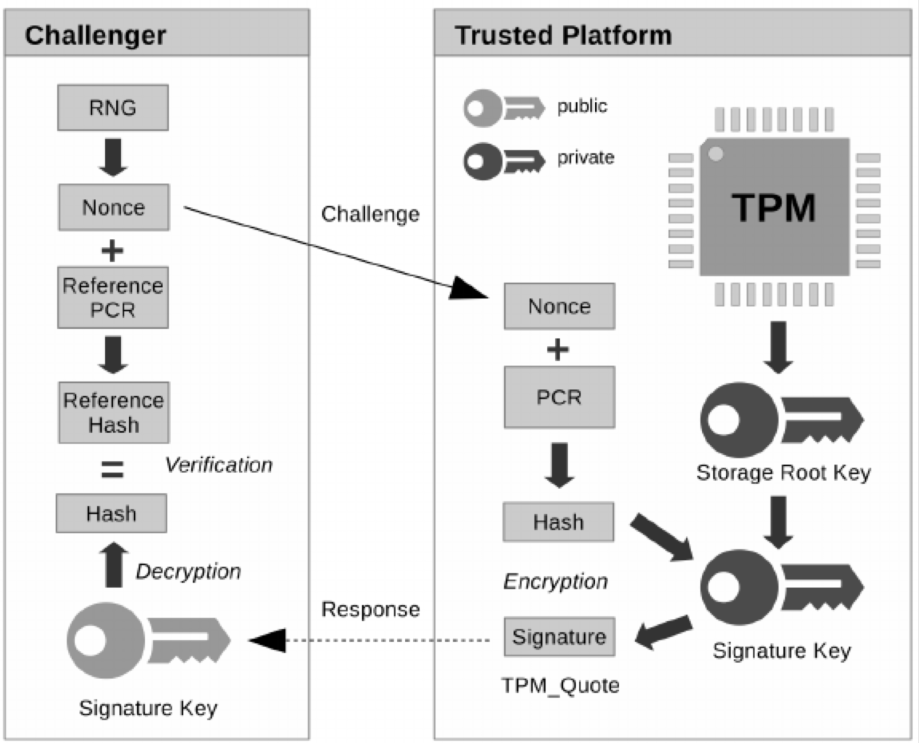
\includegraphics[width=0.5\linewidth]{tpm_attestation}}%
	\caption{Remote Attestation process}
	\label{fig:tpm_attestation}
\end{figure}

Then the platform creates a message with the nonce received previously and the existing configuration and calculates an hash value for that message. With an Attestation Identity Key (AIK), the message is then signed and sent back to the remote system, which then proceeds to decrypt the message with the \gls{ek} public part, that then compares the result with the hash of the nonce plus the configuration it had at the begining of the challenge. 

If the hashes match, the remote system can then identify the \gls{tpm} platform as a trusted platform.

\subsection{HSM – Hardware Security Modules}
\label{ssec:hsm}

\gls{hsm} \cite{hsmPaper} are physical components whose main function is to provide and store cryptographic keys used to encrypt/decrypt data inside a system. \gls{hsm}s can also perform cryptographic operations (e.g. encryption, hashing, etc.) as well as authenticate through verification of digital signatures and accelerate \gls{ssl} connections \cite{hsmThesis}.

This modules are used mainly in large environment systems (e.g. large distributed systems) where there are a lot of machines communicating with each other, therefore creating a more needed sense of security. The inclusion of this modules in these big systems is actually a good idea since \gls{hsm}s can also help servers relieve the workload caused by cryptographic operations. However \gls{hsm}s do not quite guarantee the idea of absolute security, but increment the cost of attacking the system.

Although \gls{hsm}s grant some extra level of security to a system, there's some drawbacks. One of them is the cost, where to buy one \gls{hsm} the price varies depending on the sophistication of the security, plus the cost of maintenance makes it even more expensive. Another disadvantage is the difficulty to update a software module that is already running in a functional \gls{hsm}.

\subsection{Trusted Execution Environments}
\label{ssec:tee}

A Trusted Execution Environment is an abstraction provided by both software and hardware that guarantees isolated execution of specific programs from all the other programs running on the same machine \cite{guiBorgesThesis}, including the host OS, hypervisor or even system administrators, preventing them from leveraging their priviledges and thus take advantage of the system. A \gls{tee} also grants secured storage of sensitive data, as well as remote attestation to make sure a given program runs as expected on a remote \gls{tee}. 

For a user to communicate with his program running inside an isolated environment, a key-exchange between the \gls{tee} and the user takes place. This way it is ensured both integrity and confidentiality of data during further communications.

This \gls{tee} abstraction can be achieved either by using a virtual machine monitor or by running security critical software (from whole applications to little segments of code) under protection mechanisms provided by hardware \cite{pcopThesis}. 

In the next chapters we will be looking into more dept about this hardware protection providers, that are capable of creating trusted and isolated environments in the systems nowadays.




\subsection{Discussion}
\label{ssec:tee_discussion}

Although all the approaches discussed before aim to offer better levels of security to applications, it's possible to find some differences between them. 

Between the hardware-only approaches TPM and \gls{hsm}, while \gls{tpm} is a "fixed" module, since it's typically on the motherboard, \gls{hsm} is a more flexible approach and can be added to the system after, either as an I/O device or via network. Also \gls{hsm} is more optimized to be used at the network level, and it's mainly used by banks to perform encryption of user data, while \gls{tpm} is more suited to deal with encryption of local files.

Adding to this, we also discussed hardware and software approaches. 
From the four technologies, \gls{sgx} is the one that proven to be the most reliable for our work. Comparing to ARM Trust Zone, while both really popular in today's systems, \gls{sgx} supports remote attestation while ARM's approach does not. AMD SEV does not provide protection against replaying attacks, and though it's capable of running whole \gls{vm}s, it does not support remote attestation, much like ARM's approach. It's also less used by the community than \gls{sgx}. Sanctum offers a feature that \gls{sgx} does not offer, which is protection against side-channel attacks. Although the fact that Sactum's implementation was focused on dealing with software attacks resulted in a minimal design for it's enclaves, thus being more susceptible to physical attacks. Also adding the fact that it's the less used approach from all four and it targeted RISC-V processors, made \gls{sgx} a better option.

Altough \gls{sgx} does not protect an application from side-channel attacks, it ensures hardware integrity and confidentiality of data, adding the fact that it has proven to be capable of running unmodified applications, by using recently developed frameworks.





% section introduction (end)

% ====================
% = Folder Structure =
% ====================
\section{TEE/SGX Enabled Protection Against Untrusted OSes} % (fold)
\label{sec:tee_enabled_frameworks}

A lot of applications these days depend on sensitive data to operate therefore protecting these data must be taken into account while designing the application. 

One of the things we have to think about is the size of the \gls{tcb}, and how to reduce it as much as possible without losing the operability of the system. Typically, the host \gls{os} is considered safe, trustworthy, although that is not always the case. A compromised \gls{os} can give complete access to this sensitive data, regardless of how well designed the application is. That's why this is a major security problem and must be tackled in today's systems. 

In the following subsections will be discussed how to achieve security for this particular problem, how to remove the OS from our TCB without losing functionability of the system, preferably without any major drawbacks in the system's performance. Thus we'll introduce some software techniques that can increase the security of an application against that threat.

\subsection{Virtual Ghost}
\label{ssec:virtghost}

\subsection{Flicker}
\label{ssec:flicker}


\subsection{MUSHI}
\label{ssec:mushi}


\subsection{SeCage}
\label{ssec:secage}



\subsection{InkTag}
\label{ssec:inktag}




\subsection{Sego}
\label{ssec:sego}



\subsection{Other approaches}
\label{ssec:tee_other_frameworks}

There are also other approaches that tackle the same problem of trusting the OS, making it impossible for the execution of an  application to be compromised by a malicious OS, such as 

\begin{itemize}
	\item Hardware-assisted Data-Flow Isolation (HDFI) \cite{hdfiPaper} - data isolation mechanism running on top of RISC-V that uses machine instructions and hardware to enforce isolation, by virtually extending each memory unit with an additional tag that is defined by data-flow. It grants stack protection, standard library enhancement, kernel data protection, virtual function table protection, code pointer protection and information leak prevention. It's easy to use and imposes low performance overhead, while improving security.
	
	\item Secure Channel between Rich Execution Environment and Trusted Execution Environment (SeCReT) \cite{secretPaper} - it is a framework that is focused in securing the communications between the Rich Execution Environments (REE) and the TEE built in ARM TrustZone, to add to the idea of isolation from the OS. It enables legitimate processes to use a session key in the REE, which is regarded as unsafe. To protect the key, SeCReT verifies the code's integrity and control-flow of the process every time a switch between user mode and kernel mode takes place. SeCReT's key-protection mechanism is only activated during the runtime of the process that has permission to access TrustZone, so it minimizes the performance overhead.
	
	
\end{itemize}



\subsection{Discussion}
\label{ssec:tee_frameworks_discussion}

Another conclusion about the differences of the approaches. 
 
//TODO

Virtual Ghost - 
performs well compared to previous approaches; it outperforms InkTag on five out of seven of the
LMBench microbenchmarks with improvements between
1.3x and 14.3x. For network downloads, Virtual Ghost experiences a 45% reduction in bandwidth at most for small
files and nearly no reduction in bandwidth for large files
and web traffic. An application we modified to use ghost
memory shows a maximum additional overhead of 5% due
to the Virtual Ghost protections. We also demonstrate Virtual Ghost’s efficacy by showing how it defeats sophisticated
rootkit attacks.

Protection against untrusted OSes.

Virtual Ghost [20] uses both compile-time and run-time
monitoring to protect an application from a potentially-
compromised OS, but requires recompilation of the
guest OS and application.

Flicker [40], MUSHI [56],
SeCage [37], InkTag [21], and Sego [32] protect appli-
cations from untrusted OS using SMM mode or virtual-
ization to enforce memory isolation between the OS and
a trusted application.

Trustlite, isolate software
on low-cost embedded devices using a Memory Protec-
tion Unit.

Minibox built a 2-way sandbox for x86
by separating the Native Client (NaCl) [55] sandbox into
modules for sandboxing and service runtime to support
application execution and use Trustvisor [39] to protect
the piece of application logic from the untrusted OS.

Secret builds a secure channel to authenticate the appli-
cation in the Untrusted area isolated by the ARM Trust-
Zone technology.

HDFI extend each memory
unit with an additional tag to enforce fine-grained isola-
tion at machine word granularity in the HDFI system.







% section folder_structure (end)

% ===================
% = Package options =
% ===================
\section{SGX-Frameworks and Application Support} % (fold)
\label{sec:sgx_frameworks}


The need for cloud computing is constantly growing in modern applications. It is a cost-effective and pratical solution to run large distributed applications, however the fact that it requires users to trust the cloud provider with their code and data creates some trust concerns for developers.
Although the usage of TEEs aim to tackle this problem by running and storing sensitive data on a isolated environment, protecting that data from unauthorized access. To accomplish this, the main approach is to devide the application into trusted and untrusted parts, reducing the TCB as much as possible as a way to reduce security breaches. 
In the next sections we'll discuss frameworks that can accomplish solutions to the problem described above, by working with Intel-SGX as the TEE provider, as a way to complement its regular execution.



\subsection{Network services protection approaches}
\label{ssec:sgx_network_frameworks}

Security and privacy have become one of the main concerns for both users and developers, therefore software technologies, like TLS and even anonymous networks like Tor, have become quite popular. At the same time, hardware approaches capable of providing TEEs (e.g. Intel-SGX) have also made contributions to help with this concerns. 
As these technologies are being adapted by applications, it's also believed that they can have a significant impact on networking security, since they can be used, for instance, to solve policy privacy issues in inter-domain routing, thus protecting ISPs policies. 

In \cite{torSGXPaper} it's shown that leveraging hardware protection of TEEs can grant benefits, such as simplify the overall design of the application, as well as securely introduce in-network functionality into TLS sessions. 
The same paper also presents a possible approach to reach security and privacy on a network level, by building a prototype on top of OpenSGX, that shows that SGX-enabled applications have modest performance losses compared to one with no SGX support, while significantly improving it's security and privacy.

Also at the networking security level, the usage of Network Function Virtualization (NFV) architecture by applications nowadays imply the creation of internal state as a way to allow complex cross-packet and cross-flow analysis. These states contain sensitive information, like IP addresses, user details and cached content (e.g. profile pictures), therefore should be a priority to ensure their protection from potential threats. 

To tackle this vulnerability, S-NFV has proven to be a valid approach. 
S-NFV provides a secure framework for NFV applications, securing NFV states by using Intel-SGX. S-NFV divides the NFV application in two: S-NFV enclave and S-NFV host. The enclave is responsible to store the states and state processing code, while the host deals with the rest.

In \cite{sNFVPaper} by implementing the S-NFV approach with Snort \cite{snortPaper} on top of OpenSGX was concluded that this SGX-enabled approach results in bigger overheads (aprox. 11x for gets and 9x for sets) than an SGX-disabled Snort application, at the cost of extra security.



\subsection{Application-level protection approaches}
\label{ssec:sgx_applvl_frameworks}

There are software approaches that allow unmodified applications to execute while offering security from potentially malicious OSes, achieved by isolating sensitive data from the rest. 

In addition to Graphene-SGX \ref{ssec:grapheneSGX}, approaches like Haven \cite{havenPaper}, Scone \cite{sconePaper} and Panoply \cite{panoplyPaper} offer system support, by ensure a secured way for the application to make system calls, such as implementing a library OS or a standard library, inside the enclave. 
Haven runs an entire library OS (LibOS) inside the enclave, resulting on a very large TCB. 
Scone uses sandboxing as a way to reduce TCB size due to the LibOS approach.
Panoply provides the abstraction of micro-container (micron), having only to import specific micron-libraries instead of the whole LibOS, resulting in a shorter increase of the TCB size. 

Although capable of ensuring unmodified applications a way of running on top of SGX, the increase of the TCB size has been seen as a possible vulnerability. 
Thus new approaches more focused on this TCB size problem, like Glamdring \cite{glamdringPaper} and SGX-Shield \cite{sgxShieldPaper}, have been developed lately by the community as possible alternatives to the above ones.




\subsection{Discussion}
\label{ssec:sgx_frameworks_discussion}

Haven [15] showed
that a library OS could run unmodified applications on
SGX,

thin “shim” layers, like SCONE [14] and Panoply [49] wrap 
an API layer such as the system call table.


--------


SGX frameworks and applications.

VC3 [45]
runs MapReduce jobs in SGX enclaves.

Bren-
ner et al. [17] run cluster services in ZooKeeper in an
enclave, and transparently encrypt data in transit be-
tween enclaves.

Ryoan [22] sandboxes a piece of un-
trusted code in the enclave to process secret data while
preventing the loaded code from leaking secret data.

Opaque [57] uses an SGX-protected layer on the Spark
framework to generate oblivious relational operators that
hide the access patterns of distributed queries.

The \novathesis\ class can be customized with the options listed below.



\section{Related work analysis and rational} % (fold)
\label{sec:relatedwork_analysis}

In this section we will provide some additional considerations about some of the customizations available as class options.



